\uuid{m2Ch}
\exo7id{4998}
\auteur{quercia}
\organisation{exo7}
\datecreate{2010-03-17}
\isIndication{false}
\isCorrection{true}
\chapitre{Courbes planes}
\sousChapitre{Courbes définies par une condition}

\contenu{
\texte{
$$
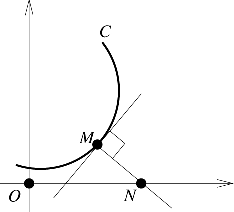
\includegraphics[width=4cm]{../images/img004998-1}
$$
 Trouver les courbes $\mathcal{C}$ telles que $MN = ON$.
}
\reponse{
La tangente ne doit pas être parallèle à $Oy$, donc on peut paramétrer
$\mathcal{C}$ sous la forme : $y=f(x)$, ce qui donne l'équation :
$$|x+yy'| = |y|\sqrt{1+y'^2} \Leftrightarrow
2xyy' = y^2-x^2.$$
(équation homogène) on obtient : $y = \pm\sqrt{\lambda x - x^2}$. Les courbes
cherchées sont des arcs de cercles centrés sur $Ox$ passant par $O$.
}
}
